\documentclass[11pt]{article}

\usepackage[UTF8]{ctex} % for Chinese 

\usepackage{setspace}
\usepackage[colorlinks,linkcolor=blue,anchorcolor=red,citecolor=black]{hyperref}
\usepackage{lineno}
\usepackage{booktabs}
\usepackage{graphicx}
\usepackage{float}
\usepackage{floatrow}
\usepackage{subfigure}
\usepackage{caption}
\usepackage{subcaption}
\usepackage{geometry}
\usepackage{multirow}
\usepackage{longtable}
\usepackage{lscape}
\usepackage{booktabs}
\usepackage{natbib}
\usepackage{natbibspacing}
\usepackage[toc,page]{appendix}
\usepackage{makecell}

\title{老子}
\date{}

\linespread{1.5}
\geometry{left=2cm,right=2cm,top=2cm,bottom=2cm}

\begin{document}

  \maketitle
  
  \begin{figure}[H]
    \centering
    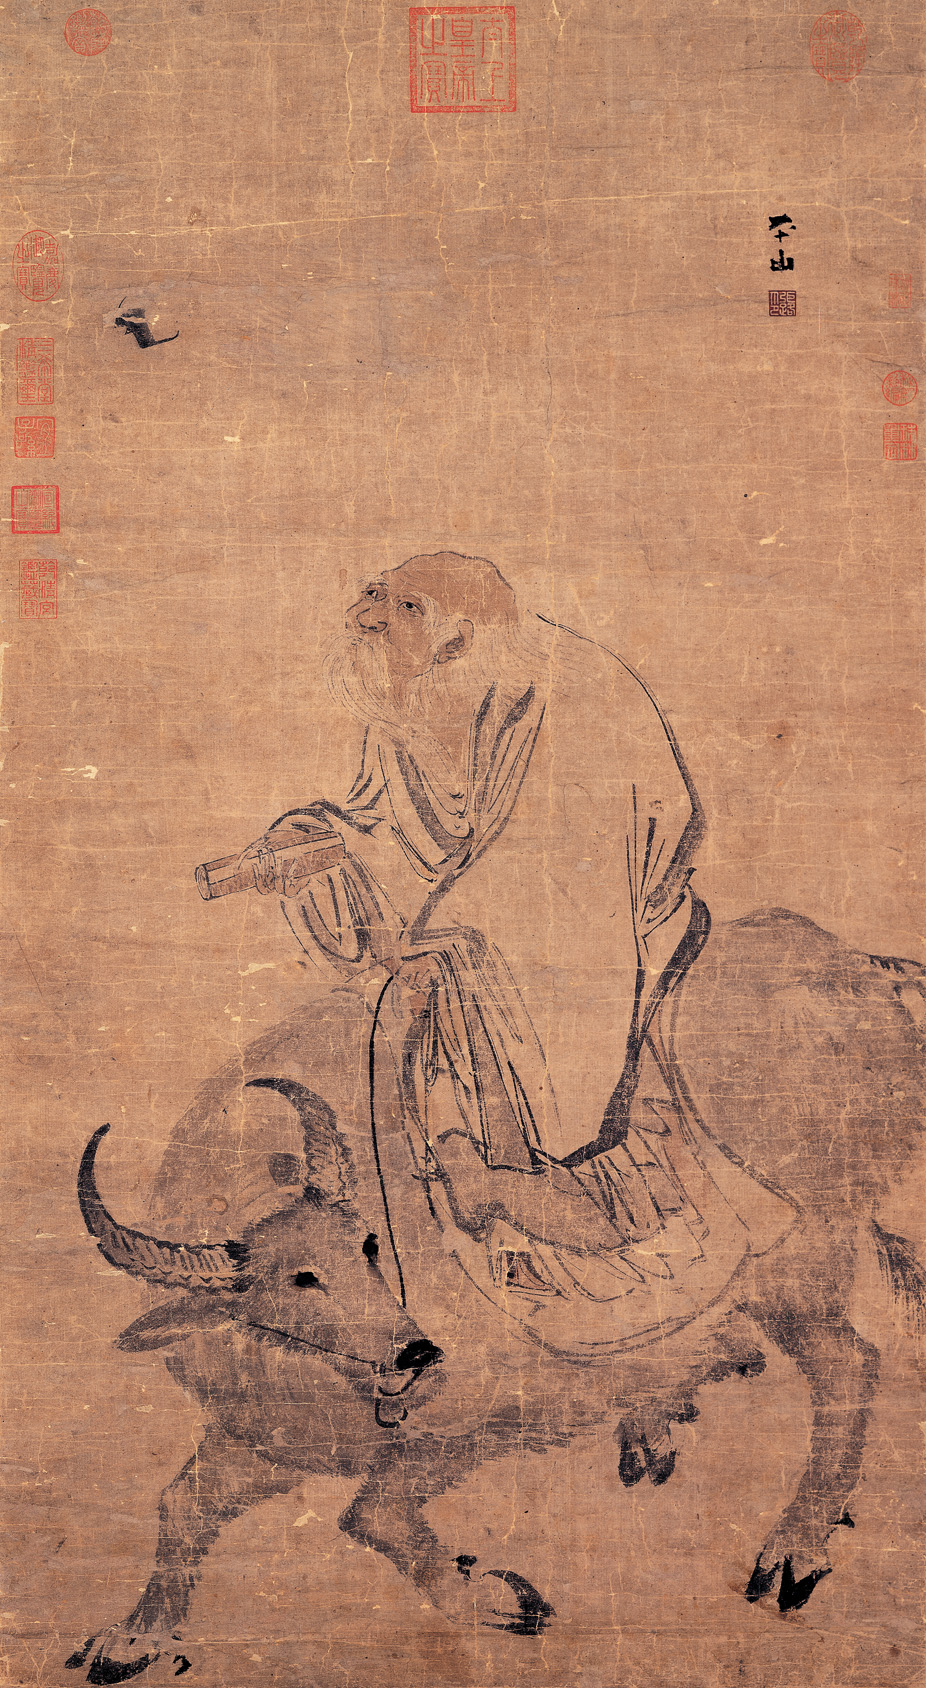
\includegraphics[height=0.7\textwidth]{../Figures/LaoZi.jpg}
    \caption{老子像。台湾国立故宫博物院藏。}
  \end{figure}

  \newpage
  
  \linenumbers

老子姓李名耳,楚之苦县人,早年任周吏,管理藏书。
孔子曾问礼于老子,对其异常倾佩,以为人中龙凤。
后老子云游四方,遍观人间疾苦,悟得大道,遂西出函谷,行将飞升。
关令尹喜恐老子隐后,大道不传,强留其著书。
老子遂作《道德经》五千言遗之,而后一路西行。
途径戎狄之国,见其民堕于外道邪法,甚悲悯之。
遂举大神通,欲化之以正法大道。
又恐夷民粗鄙愚笨,难解大道。
遂作浮屠之法传之。
有戎国王子乔达摩·悉达多,得老子牙慧,竟成佛陀,显赫至今。
而老子深藏功名,拂衣而去,羽化飞升。
今人所供奉之太上老君,即是老子。

\newline

以上所述老子生平出自民间传说,基本属于虚构,但“深藏功名,拂衣而去”,却非妄言。
老子系中国文化一甚大人物。
据说世界各类图书的销量榜单上,《道德经》排进前三,且各种乱七八糟的译本层出不穷。
汉代道教兴起后,老子更是坐上了全宇宙第一把交椅。
然此等显赫人物,竟神龙见首不见尾。
其身世、时代皆成问题,就连姓名亦存疑窦。
老子其书其人,真伪先后之辩,积讼已久。
历代学者群言兹繁,鲜有一较为确定之结论。
写出这般作品却不署名,可见其不为名利所绊,真真天下第一等潇洒人物。
不信,试观今日,哪位敢写篇东西不注明作者、声明版权所有?
连我这种没受过教育的货色写篇小论文,尚且要写清楚作者是谁,甚至还要注明所属单位,免得和别人重名。
想想老子,看看自己,真愧煞人也。

\newline

\section{道}
万物流变不息,皆不能久常。
《道德经·二十三章》谓:

\textit{飘风不终朝,骤雨不终日。孰为此者?天地。天地尚不能久,而况於人乎?}

换言之,凡属于客观物质世界者,皆处于一不断变化之状态。
而万物变化所依循之规律,系一超出物质世界之存在,故可久可常。
此种规律,老子名之曰“道”。
《道德经·二十五章》谓:

\textit{有物混成,先天地生。寂兮寥兮,独立而不改,周行而不殆,可以为天地母。吾不知其名,强字之曰道,强为之名曰大。大曰逝,逝曰远,远曰反。故道大,天大,地大,人亦大。域中有四大,而人居其一焉。人法地,地法天,天法道,道法自然。}

道为超越物质世界之久常存在,为万物运行之永恒规律,遍于万物而无终止,故曰“独立而不改,周行而不殆”。
物质世界依照道来运行,道对物质世界起范铸作用,故曰“道法自然”。

\newline

道系万物之总原理,故不可言说。
《道德经·一章》谓:

\textit{道可道,非常道;名可名,非常名。}

盖可以语言描述之规律,势必有其作用范围。
可言说之原理,其作用范围必为某类事物。
而道之作用范围为一切事物。故无法对道作正面诠释,言其是什么;而只能作否定性断语,即道不是什么。
故曰“道可道,非常道”。
盖凡命名,系由一组条件限定范围,遂有“此”和“非此”之区分。
而道之运行遍在于万物,无从为之限定范围,无从寻其反面,故不可正面定义。
故曰“名可名,非常名”。

\newline

道之内容为反。
《道德经·四十章》云:

\textit{反着道之动。}

每一事物或性质均有其反面。
事物发展至于某一极端,则必然向另一相反极端逐渐转变,此即所谓“反”。
“动”指运行。
故“反”为道之运行表现,为道范铸万物之效用。
  
\section{无为}
万物悉在变逝之中,皆无实性,故皆为不可凭依者。
由此老子主张无为,即自觉心不陷溺于任何外在事物。
事物均在“反”中,故不可执,执则必为陷溺。
心合于道,观万物于反中变逝,而不溺于物,此即无为之境界。
换言之,自觉心不依靠任何客观事物,方能超越万物,达到道之境界,遂观万殊事物之永恒理序。
《道德经·十六章》云:

\textit{致虚极,守静笃。万物并作,吾以观复。夫物芸芸,各复归其根。归根曰静,静曰复命。复命曰常,知常曰明。不知常,妄作凶。知常容,容乃公,公乃全,全乃天,天乃道,道乃久,没身不殆。}

\newline

自觉心脱离乃至于超越客观事物,达到无为之境界,得知大道之本质,朗照万物之根本。
此说类似佛家舍离之说。
通晓“道”之自觉心,已然超越万物,独立于物质世界,即所谓“跳出三界外,不在五行中”,则人之自觉脱离物质世界乃一自然结论。
佛学初入中国,假称老子化胡为佛,便基于此。

\newline

然而佛陀与老子终属殊途。
佛教判物质世界为虚妄迷幻。
自觉心超越万物,遂破此虚妄。
老子则无否定物质世界之倾向。
依照老子,自觉心既升入超越境界,朗照万物,遂可由中生出对客观物质世界之支配力,即是“无为而无不为”。
《道德经·三十七章》载:

\textit{道常无为而无不为。侯王若能守之,万物将自化。化而欲作,吾将镇之以无名之朴,镇之以无名之朴,夫将不欲。不欲以静,天下将自定。} 

换言之,佛陀欲以自觉心之超越性脱离物质世界之束缚,而老子欲以此支配物质世界。
后世道教致力于采药炼丹、钻研方术、探究医理,追求长生不老、羽化成仙、呼风唤雨、撒豆成兵,遂由此兴。
  
\section{守柔}
无为之终极目的在于观道。
道乃物质运行之总规律,其内容曰反。
既知道而明反,则可获得对物质世界之支配力量。
此种力量,即为“守柔”。

\newline

柔能胜强,故守柔方为真正强大。
《道德经·七十六章》谓:

\textit{人之生也柔弱,其死也坚强。草木之生也柔脆,其死也枯槁。故坚强者死之徒,柔弱者生之徒。是以兵强则灭,木强则折。强大处下,柔弱处上。}

\newline

柔弱之支配力,其依据在于反。
万物依道运行,时时皆反。
一切存在皆处于自身否定之过程中。
事物发展至极点,不可避免要变为其反面。
故人若自恃勇力,无论其力量如何强大,其运用结果必然是走向衰弱。
而自守柔弱,即预先居于强大之反面,自然逐渐强大而不至于衰竭。
一言以蔽之,人若欲如何,必先居于此如何之反面,南辕正所以取道北辙,欲强大则需守柔弱,欲擒之则需先纵之。
《道德经·三十六章》载:

\textit{将欲歙之,必故张之;将欲弱之,必故强之;将欲废之,必故兴之;将欲取之,必故与之。是谓微明。柔弱胜刚强。鱼不可脱於渊,国之利器不可以示人。}
  
\newline

守柔之至人,不陷于任何事物而能支配一切事物,于物质世界有不竭之支配力量。
老子常以婴儿比喻此等至人。
盖有大智慧之人,依照物极必反之原理,往往看似愚笨,如婴儿般无知。
此即所谓大智若愚。

\newline

至此,老子之学已近乎兵法韬略,似乎以获得无穷支配力量为纲。
然而欲获得支配万物之力量,自觉心需达到一超越境界,即知反明道。
欲达此等境界,自觉心必须不溺于任何事物。
既然不以一切事物为意,此等支配事物之力量自为无用。
换言之,一旦欲以无为守柔之力量支配事物,自觉心遂陷入其中,则不能明道,亦不能有支配力量。

\section{自我境界}
支配万物力量之发用与获得此力量相矛盾,则自觉心实际上不能于物质世界有任何作为。
如此,面对万千世界,自觉心究竟应采取何种态度?
倘判世界为虚妄,则自觉心应求破此迷幻。
此为佛陀之学。
反之,则自觉心只能观赏事物之自然运行,不能作出任何干涉。
此实为肯定人之生命感,肯定人之感性,为一艺术之境界,美学之境界。

\newline

对此自我境界问题,老子几乎没有正面回答。
然《道德经》无言世界为虚妄之语,似支持观赏世界之态度,肯定人之生命感性。
老子常以婴儿比喻此等至人,盛赞其生命力,与此相合。
《道德经·五十五章》载:

\textit{含德之厚,比於赤子。毒虫不螫,猛兽不据,攫鸟不搏。骨弱筋柔而握固。未知牝牡之合而朘作,精之至也。终日号而不嘎,和之至也。知和曰常,知常曰明。益生曰祥。心使气曰强。物壮则老,谓之不道,不道早已。}

\newline

老子论及自我境界问题,所否定者多,亦可佐证其观赏世界之态度。

\newline

首先,老子否定人之物质欲求。
《道德经·十二章》载:
\textit{五色令人目盲;五音令人耳聋;五味令人口爽;驰骋畋猎,令人心发狂;难得之货,令人行妨。是以圣人为腹不为目,故去彼取此。}

此章否定形躯欲求之满足,谓之为有害无益。
盖形躯亦为万物之一,故亦循道而行。
倘为求养生而满足欲望,追求“五色”“五音”“五味”,只会得到相反之结果,反而害生。
故圣人养生,只满足生活之基本需求而不溺于物质欲求。

\newline

其次,老子否定德性,与孔孟相左。
《道德经·十八章》谓:

\textit{大道废,有仁义;智慧出,有大伪;六亲不和,有孝慈;国家昏乱,有忠臣。}

《三十八章》更是抨击仁义礼智诸德:

\textit{故失道而后德,失德而后仁,失仁而后义,失义而后礼。夫礼者,忠信之薄,而乱之首。}

德、仁、义皆为失道后逐步堕落之产物,而礼更是堕落之极致。
由此,老子对德性之否定已甚明显矣。

\newline

再次,老子否定认知,视知识、技术、文化为堕落。
《道德经·五十七章》云:

\textit{天下多忌讳,而民弥贫;人多利器,国家滋昏;人多伎巧,奇物滋起;法令滋彰,盗贼多有。}

引文不仅否定自然科学和技术,连社会文化、制度一并否定。
《道德经·六十五章》又载:

\textit{古之善为道者,非以明民,将以愚之。民之难治,以其智多。故以智治国,国之贼;不以智治国,国之福。}

此节否定“智”,直言其为国贼。
可见,老子对认知活动亦持否定态度。

\newline

至此,形躯、德性、认知皆被否定。
老子亦不判物质世界为恶。
则自觉心于世界,仅能持观赏态度,一任其自然流动。
  
\section{政治理论}
春秋时期,礼崩乐坏,诸侯混战,社会动荡。
如何重建社会秩序为甚重要之课题,诸子于此多有论述。
老子之政治理论,基于物极必反之原理。
欲使国家得治而精心设计各种制度、构建官僚体系、编撰律法政令。
如此钻营,终将产生与原目的相反之结果。
换言之,国家之混乱,其根源在于政治秩序,在于社会、文化之发展。
唯有尽数破之,方能使国家承平。
《道德经·八十章》曰:

\textit{小国寡民。使有什伯之器而不用;使民重死而不远徙;虽有舟舆,无所乘之;虽有甲兵,无所陈之。使人复结绳而用之。至治之极。甘其食,美其服,安其居,乐其俗,邻国相望,鸡犬之声相闻,民至老死不相往来。}

此一蓝图,绝非开历史的倒车,退回原始社会。
“什伯之器”、“舟舆”、“甲兵”皆有而不用,况又能“甘其食,美其服,安其居,乐其俗”,此非原始社会之野蛮状况,而为看似野蛮之文明境界。
以物极必反之原理,此为“大文明若野蛮”也,是社会发展至终极,遂抛弃无价值之体制、文化,使人民淳朴豁达、安居乐业之最高境界。

\end{document}